\documentclass[11pt,letter]{article}
\usepackage[top=1.00in, bottom=1.0in, left=1.1in, right=1.1in]{geometry}
\renewcommand{\baselinestretch}{1.1}
\usepackage[
singlelinecheck=false % <-- important
]{caption}
\usepackage{hyperref}%helps with the email address 
\usepackage{graphicx} %including pictrures 

\def\labelitemi{--}
\parindent=0pt

\def\labelitemi{--}
\parindent=0pt

\newenvironment{smitemize}{
\begin{itemize}
  \setlength{\itemsep}{0pt}
  \setlength{\parskip}{0.8pt}
  \setlength{\parsep}{0pt}}
{\end{itemize}
}

\graphicspath{ {./protPhotos/} }% tell latex where to find photos 

\begin{document}
\bibliographystyle{/Users/Lizzie/Documents/EndnoteRelated/Bibtex/styles/besjournals}
\renewcommand{\refname}{\CHead{}}

\title{Protocol for bcvin set-up and monitoring}
\date{ }
\maketitle
\tableofcontents


\section{Choosing Vines}

Varieties sampled: Merlot, Pinot noir, Chardonnay, Riesling, Sauvignon blanc, Syrah (Shiraz), Cabernet sauvignon \\
Arterra sites: Whitetail, McIntyre, Dark Horse, NK'MIP Cellars \\
Quail's Gate sites: Quail's Gate Estate vineyard, Mannhardt \\

Using the maps and rootstock information provided we chose the blocks withe the following considerations in mind:
\begin{smitemize}
\item Sample all of our target varieties.
\item Chose blocks of different varieties near each other if possible to reduce walking distance/time. 
\item If a vineyard had multiple blocks of a variety and the blocks were different parts of the vineyard, we sampled one block in each general area to capture environmental variation within the site. If the blocks are close together, we chose to sample just one block.
\item If we sampled multiple blocks of a variety in a vineyard, we would sample 24 vines in each block rather than 36 to reduce time.
\item We preferentially chose blocks with common rootstocks - 3309, 101-14, S04 - in order to reduce effect of rootstock.
\item We avoided blocks with unknown clones or varieties and were able to avoid all of the self-rooted blocks except one (Dark Horse block G, the other Pinot noir block was recently planted).
\item When weather station locations were known, we chose rows or blocks near them.
\item Within blocks, we aimed to capture environmental variation in block, keeping in mind time needed to walk between location. Often this meant that we would sample at the bottom and top of block in the same rows if we flagged 24 plants. If we flagged 36, we would add a middle location in a different set of rows. 
\item We sampled 6 plants per row in each location. We aimed for plants to be next to each other but sometimes had to skip plants if they were too young or if they did not have a cordon with 2 spurs/cane with 2 buds.
\item Flagged vines are at least 6 plants in from the end of the row so we avoid edge effects.
\item We always chose to sample two rows next to each other in each location so there were 12 plants (6 per row) in each location.
\item 36 or 24 vines were flagged per block - if we need to reduce numbers, we will not flag less than 16 per block.

\end{smitemize}

Tip: If you are not flagging all the buds at once, flag the final bud/spur as this one will always be monitored. Doing this saves time because otherwise you may have to move the flag to another spur.

\section{Choosing Buds}

\begin{figure}%this will always show at this point 
  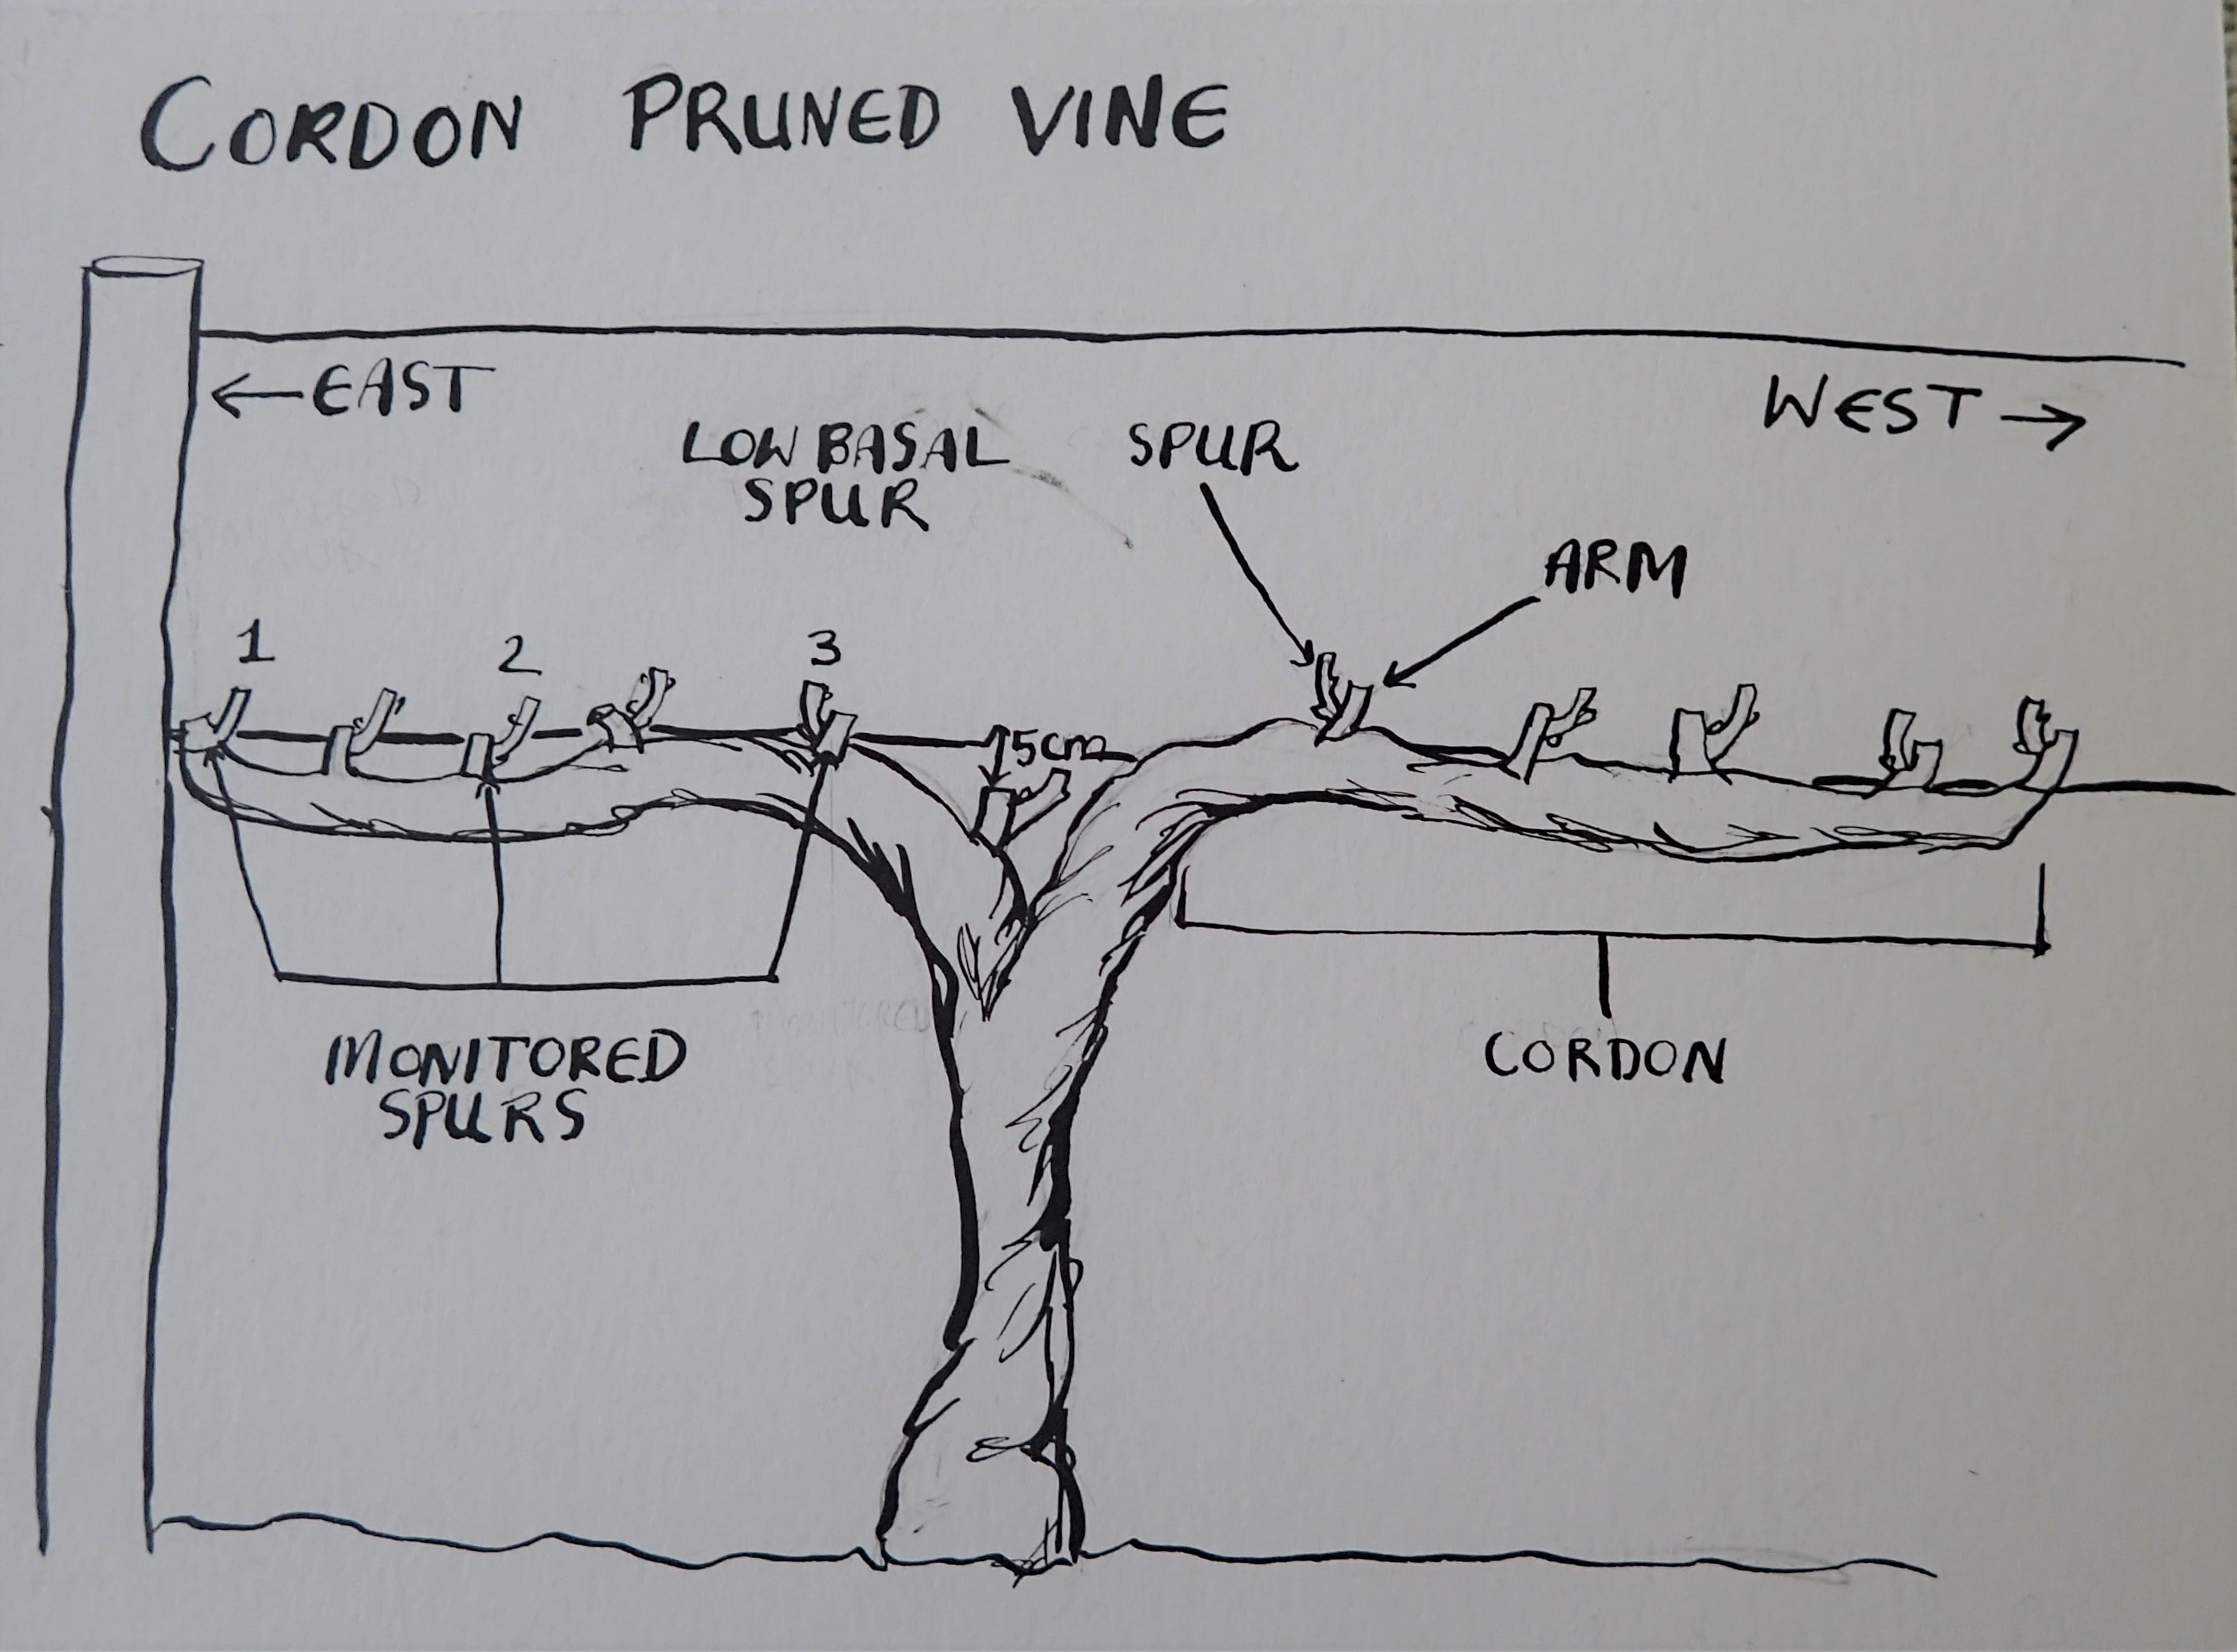
\includegraphics[width=\linewidth]{CordonPruned.jpg}
  \caption{A diagram of a cordon pruned vine, showing which spurs we would monitor. Buds were numbered from east to west or south to north, and any spur that's base was more than 5cm below the wire the cordon was trained on was not sampled.}
  \label{fig:CordonPruned}
\end{figure}

\begin{figure}%this will always show at this point 
  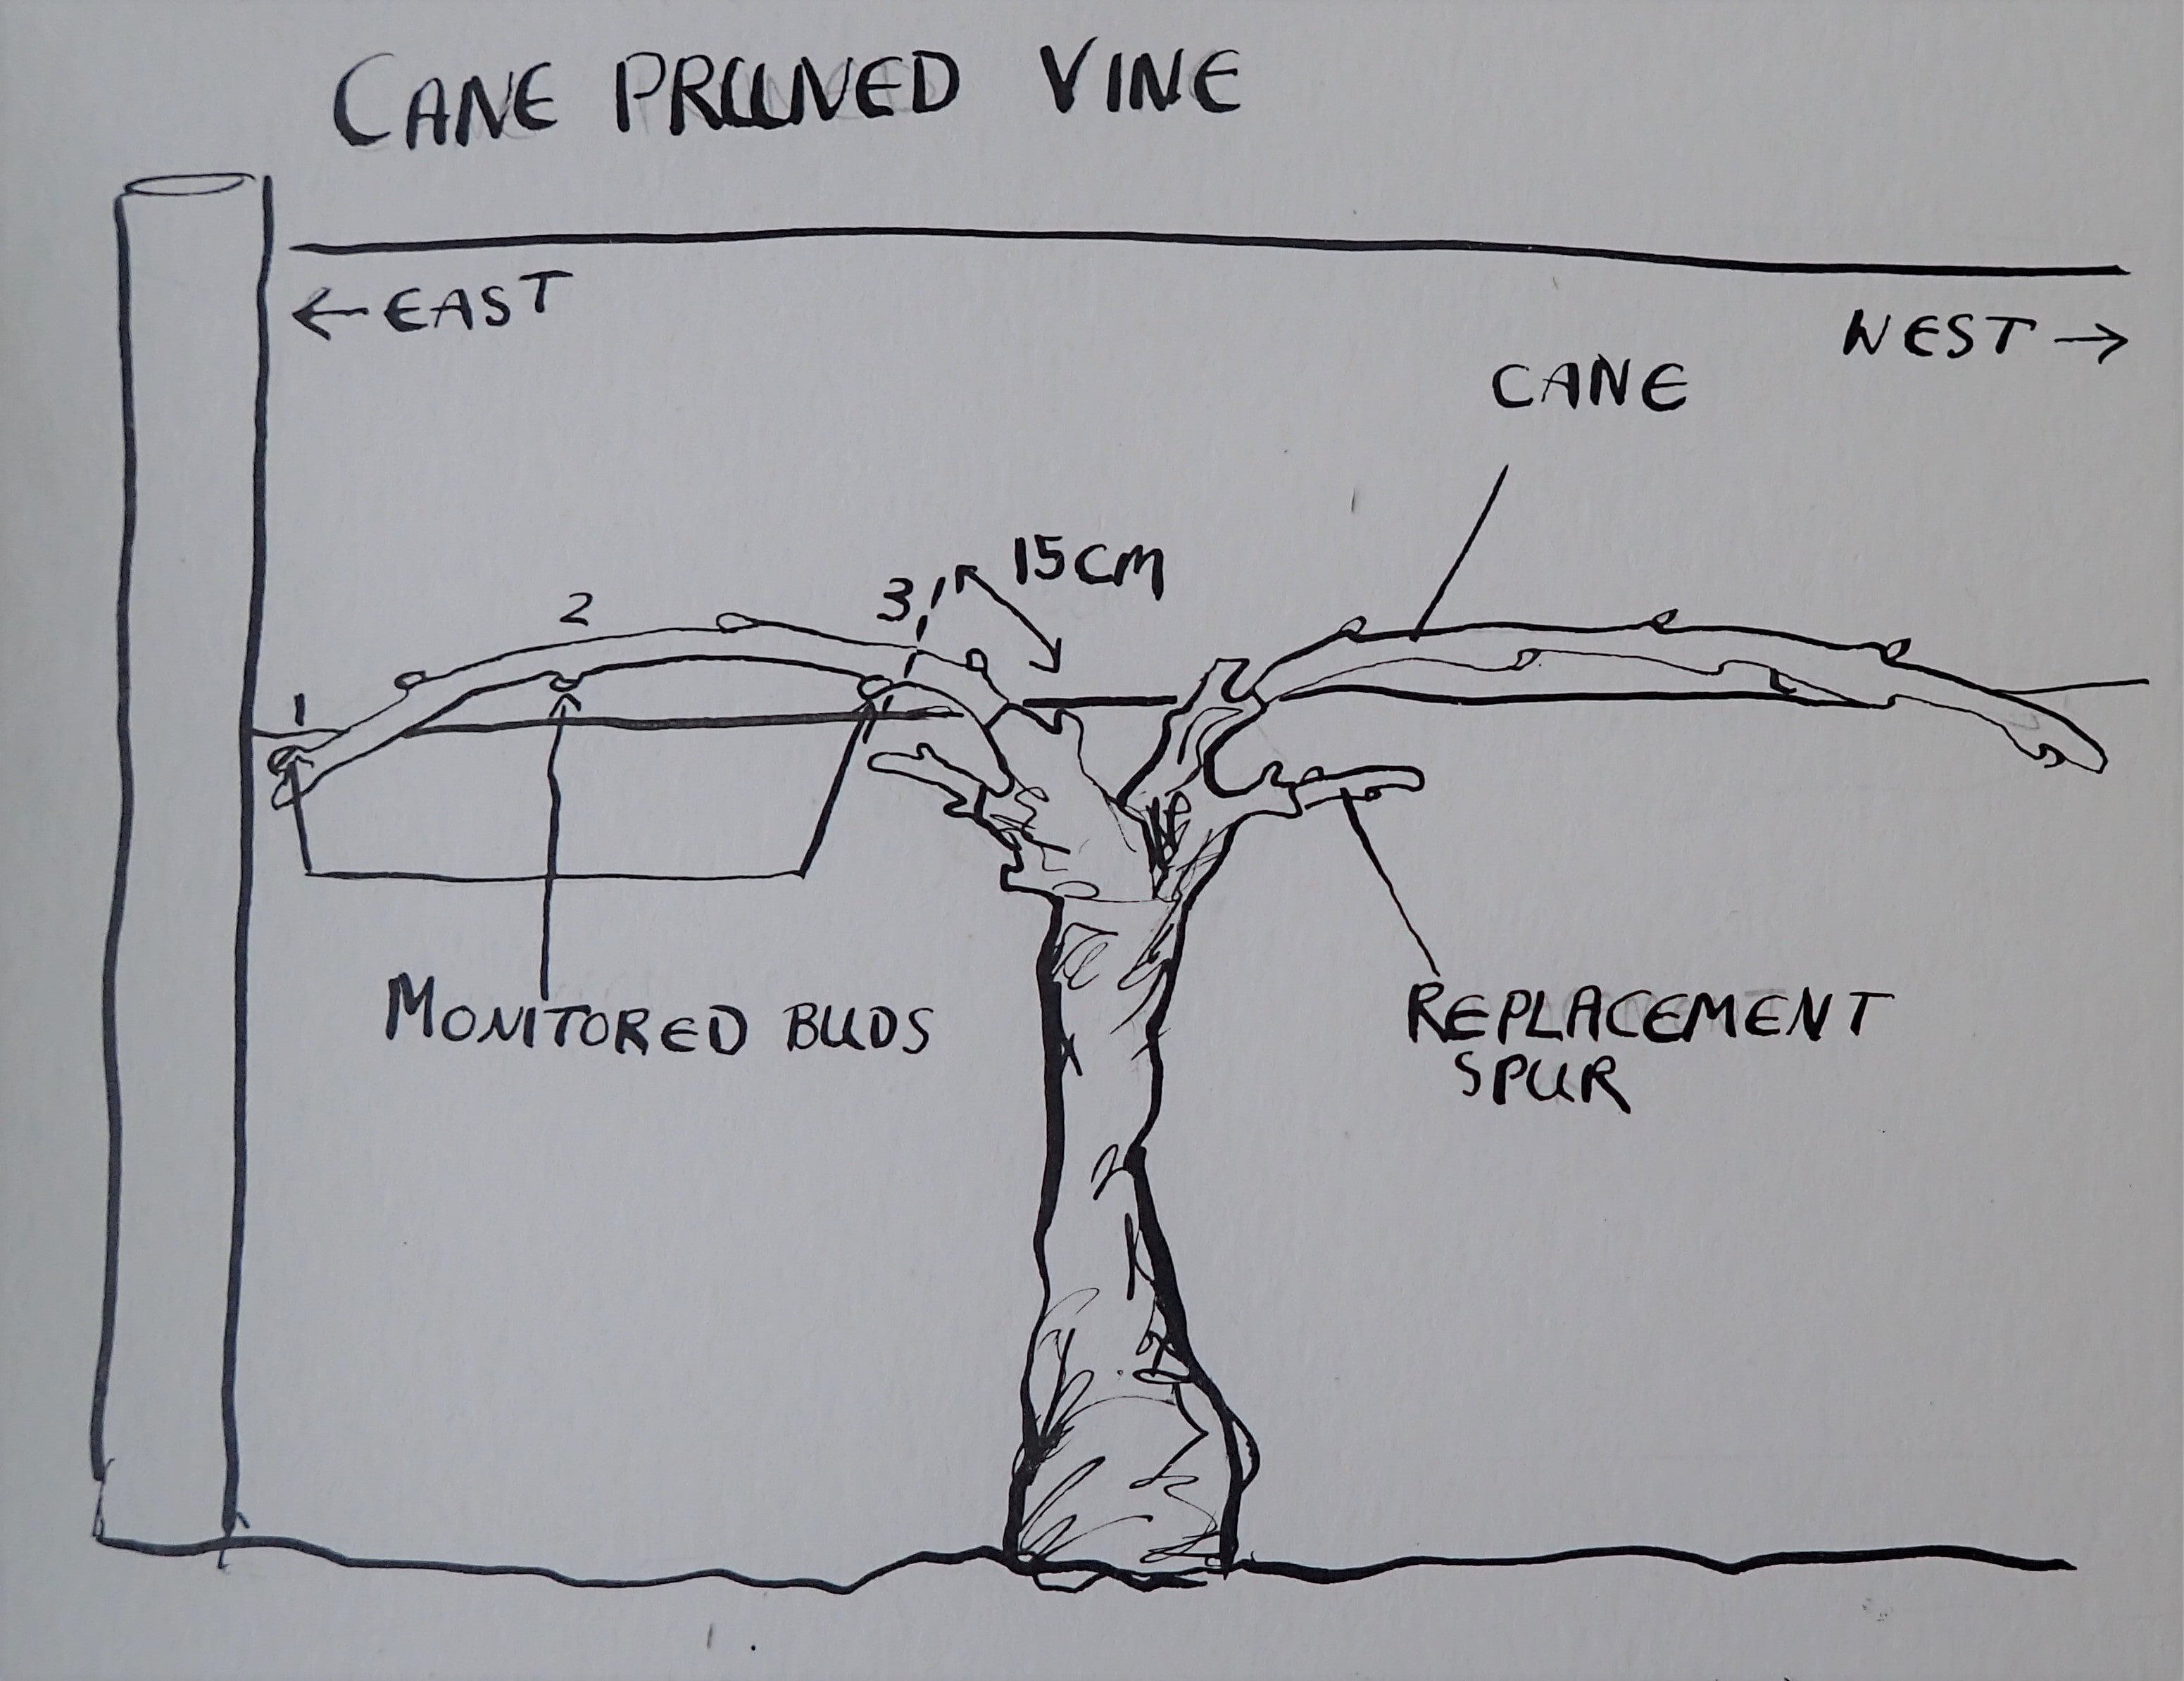
\includegraphics[width=\linewidth]{CanePruned.jpg}
  \caption{A diagram of a cane pruned vine, with the buds we would monitor and their numbering shown. Note that we do not sample buds too close to the head of the vine.}
  \label{fig:CanePruned}
\end{figure}

\begin{figure}%this will always show at this point 
  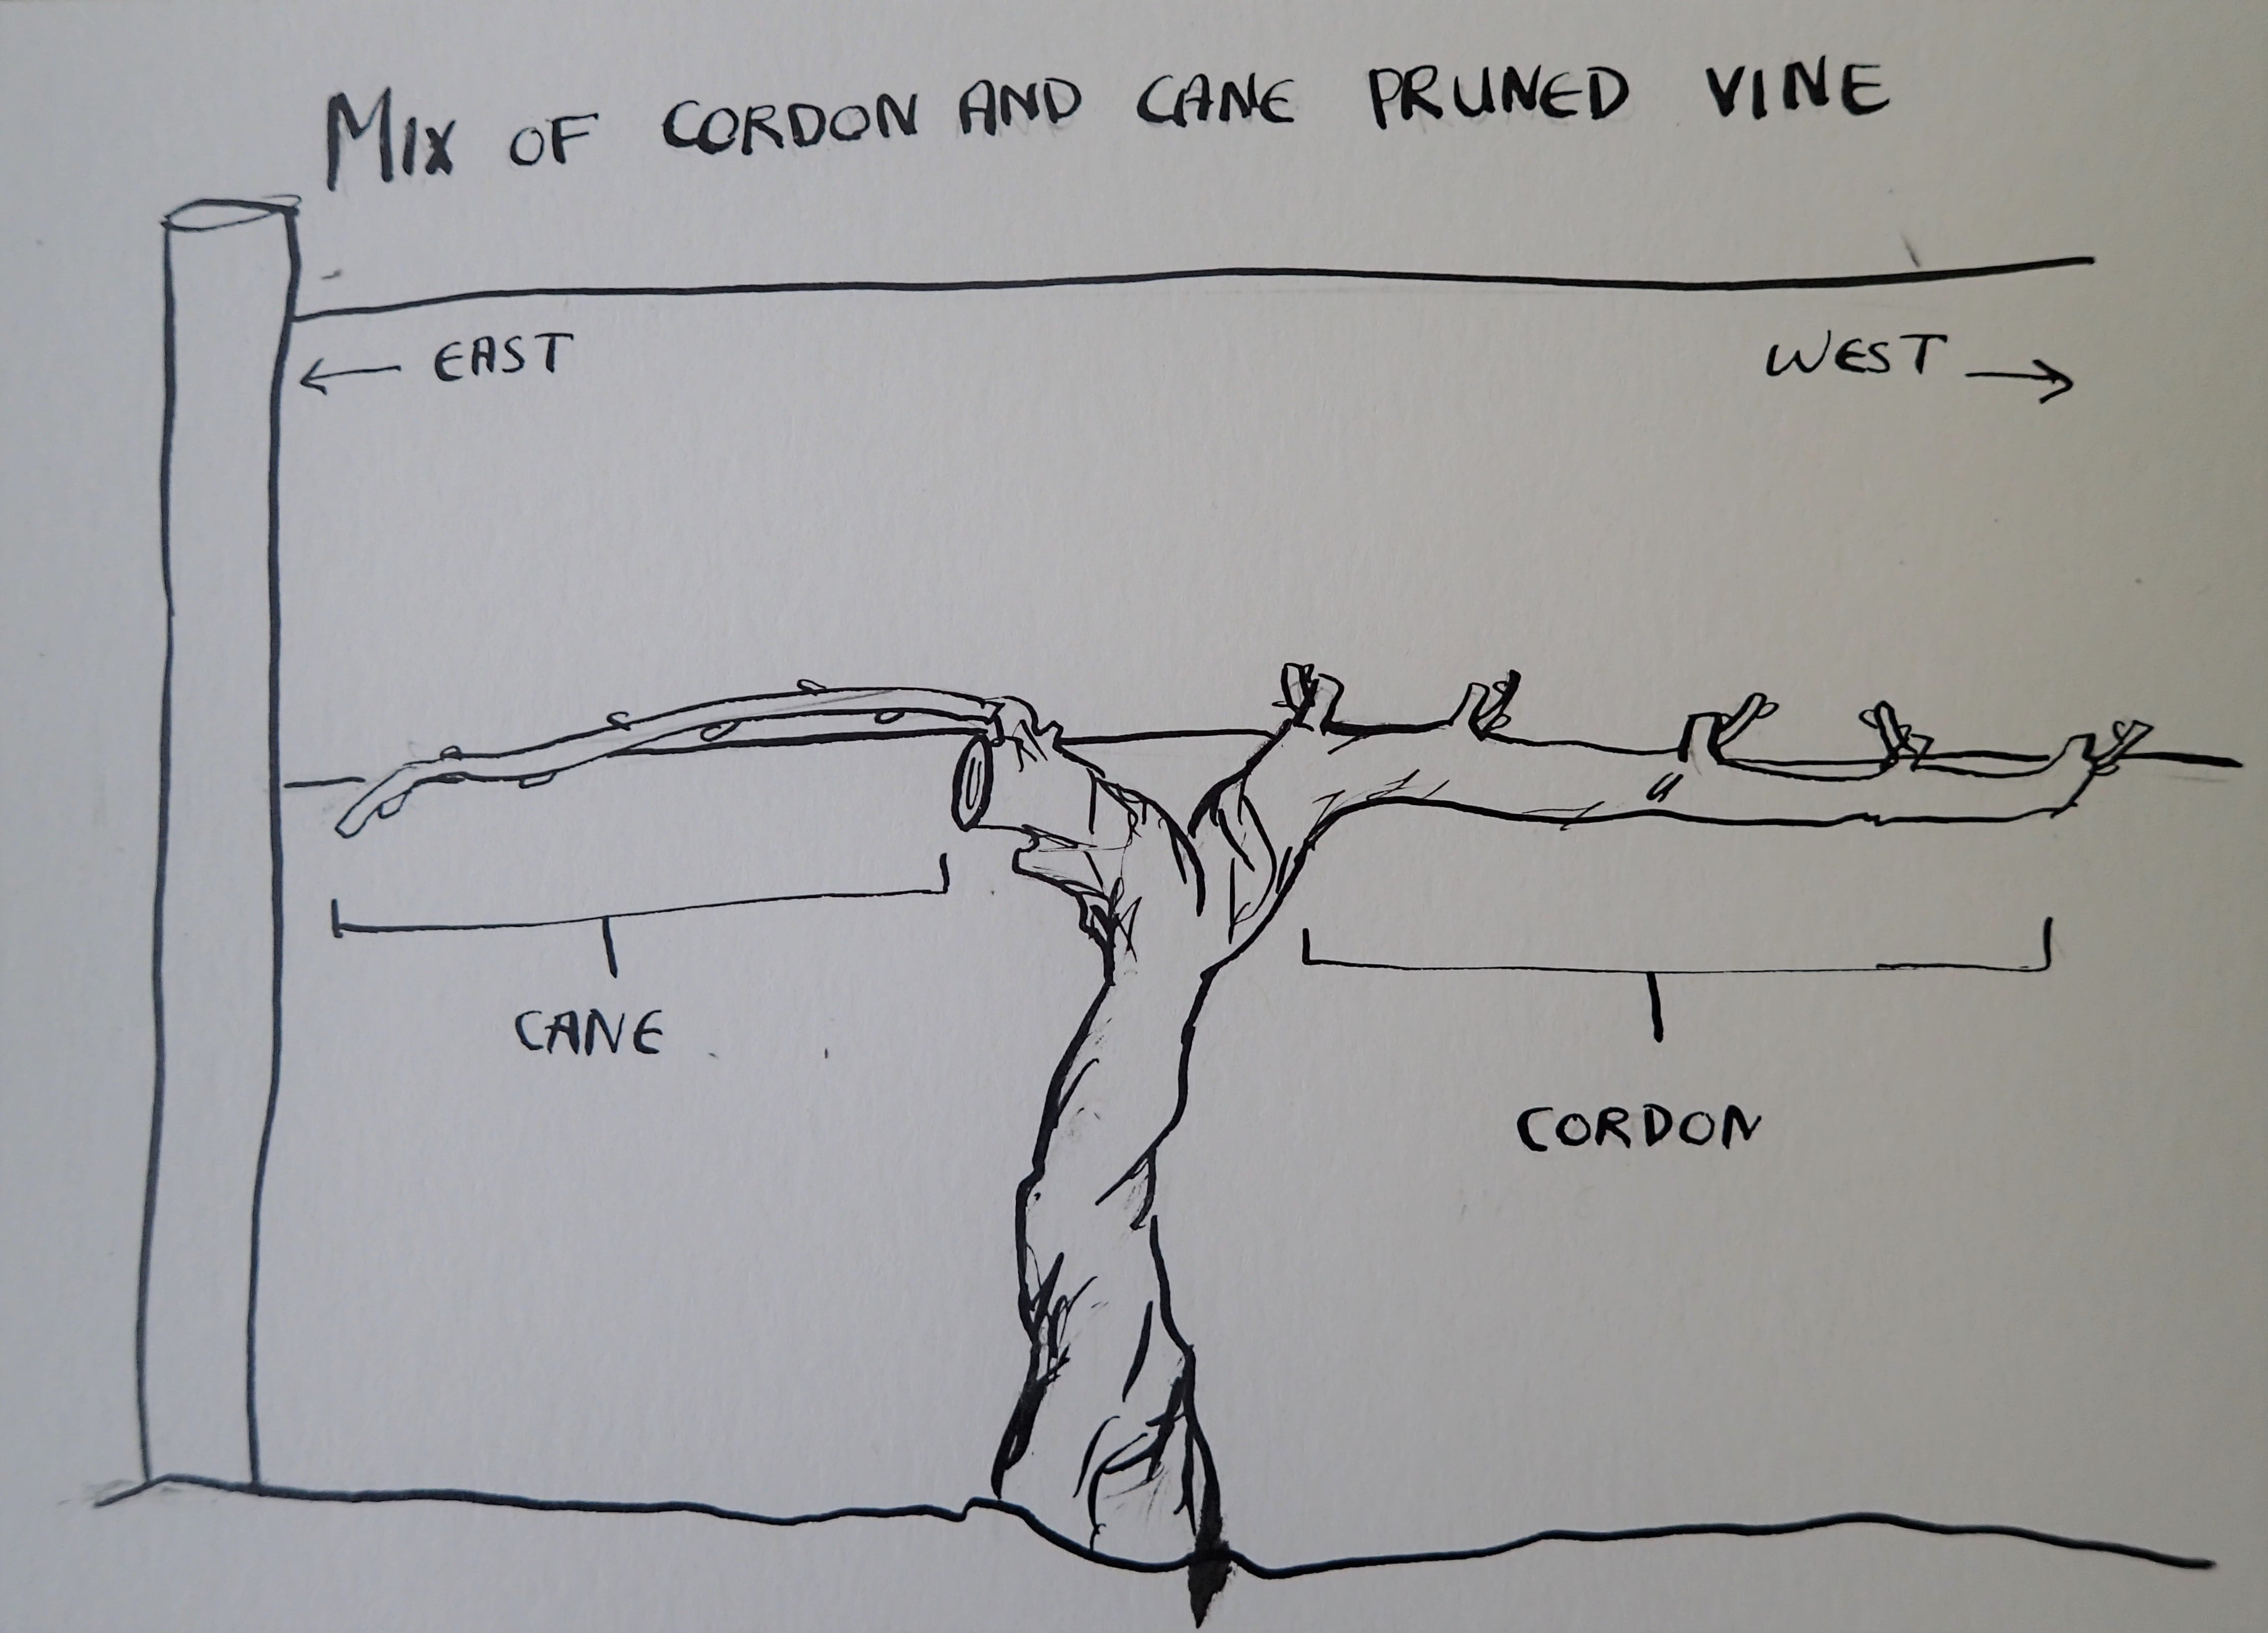
\includegraphics[width=\linewidth]{CaneCordonMix.jpg}
  \caption{When there is both a cordon and a cane, you we sample the cordon. The only time we would chose the cane rather than the cordon is if the cordon does not have enough spurs to sample.}
  \label{fig:CordonCane}
\end{figure}

\begin{figure}%this will always show at this point 
  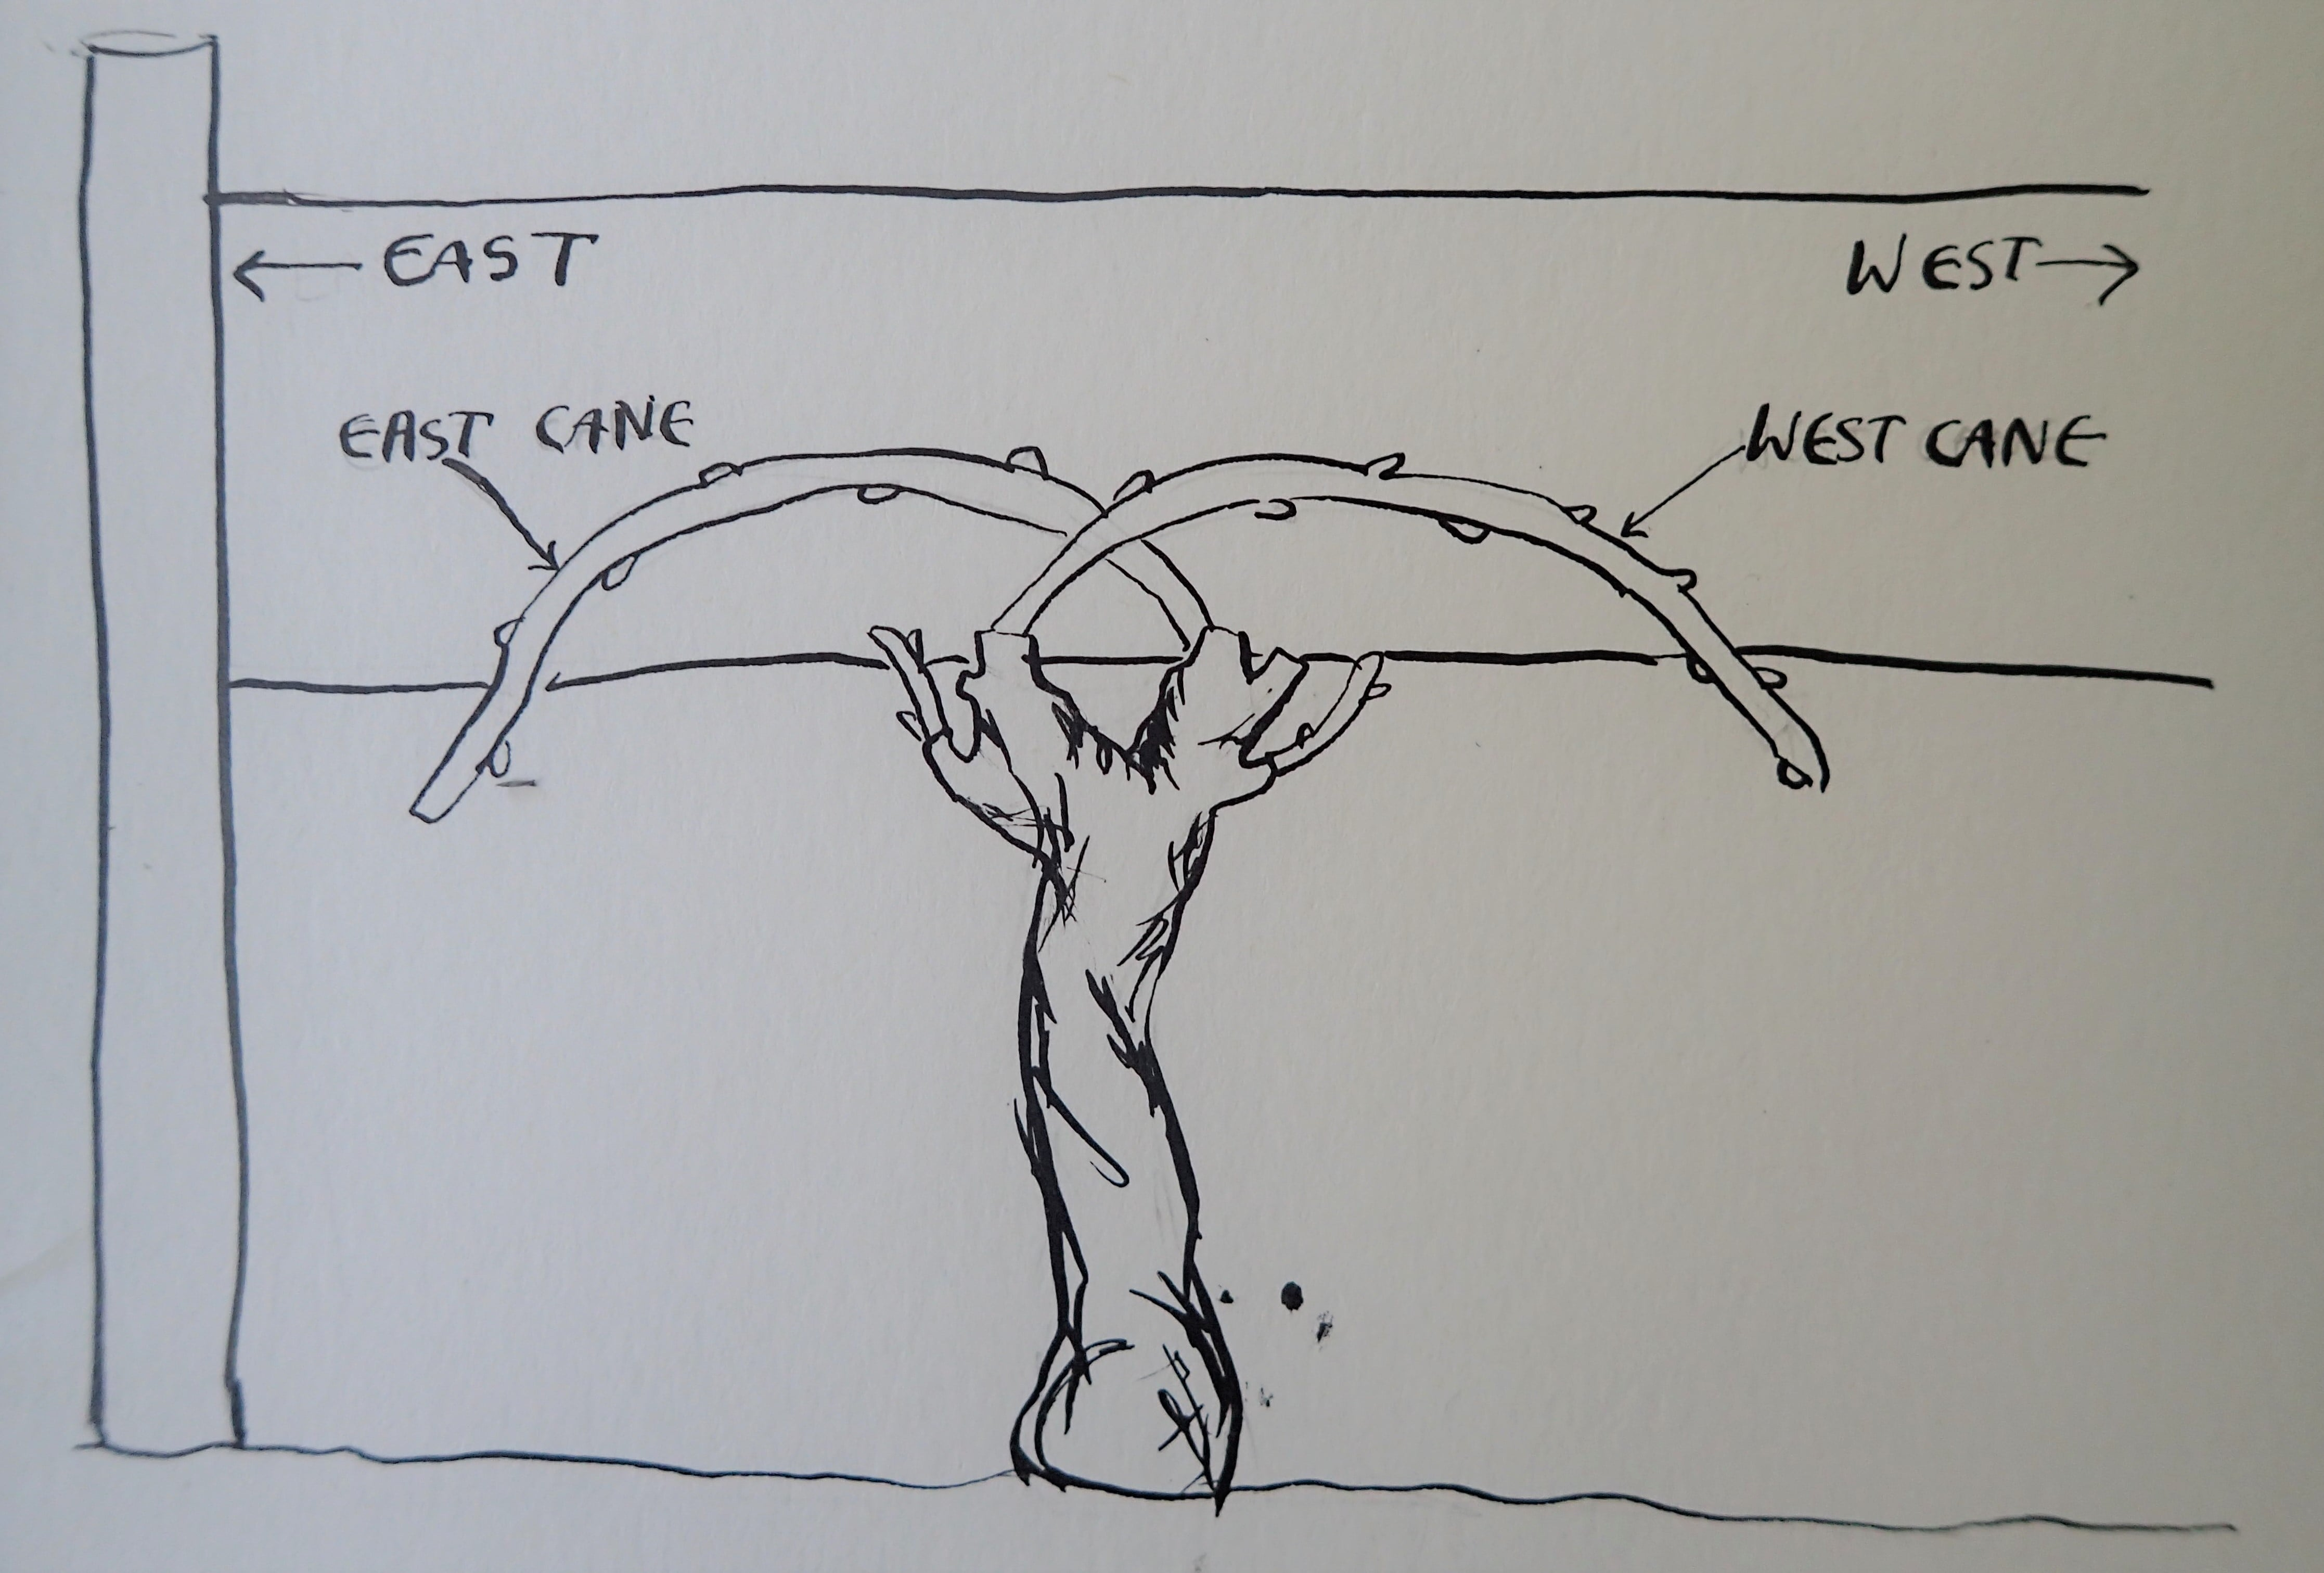
\includegraphics[width=\linewidth]{CaneCrossing.jpg}
  \caption{Sometimes the canes cross. If they do, we use the end of the cane to decide which side is east/west or north/south.}
  \label{fig:CaneCrossing}
\end{figure}

\begin{figure}%this will always show at this point 
  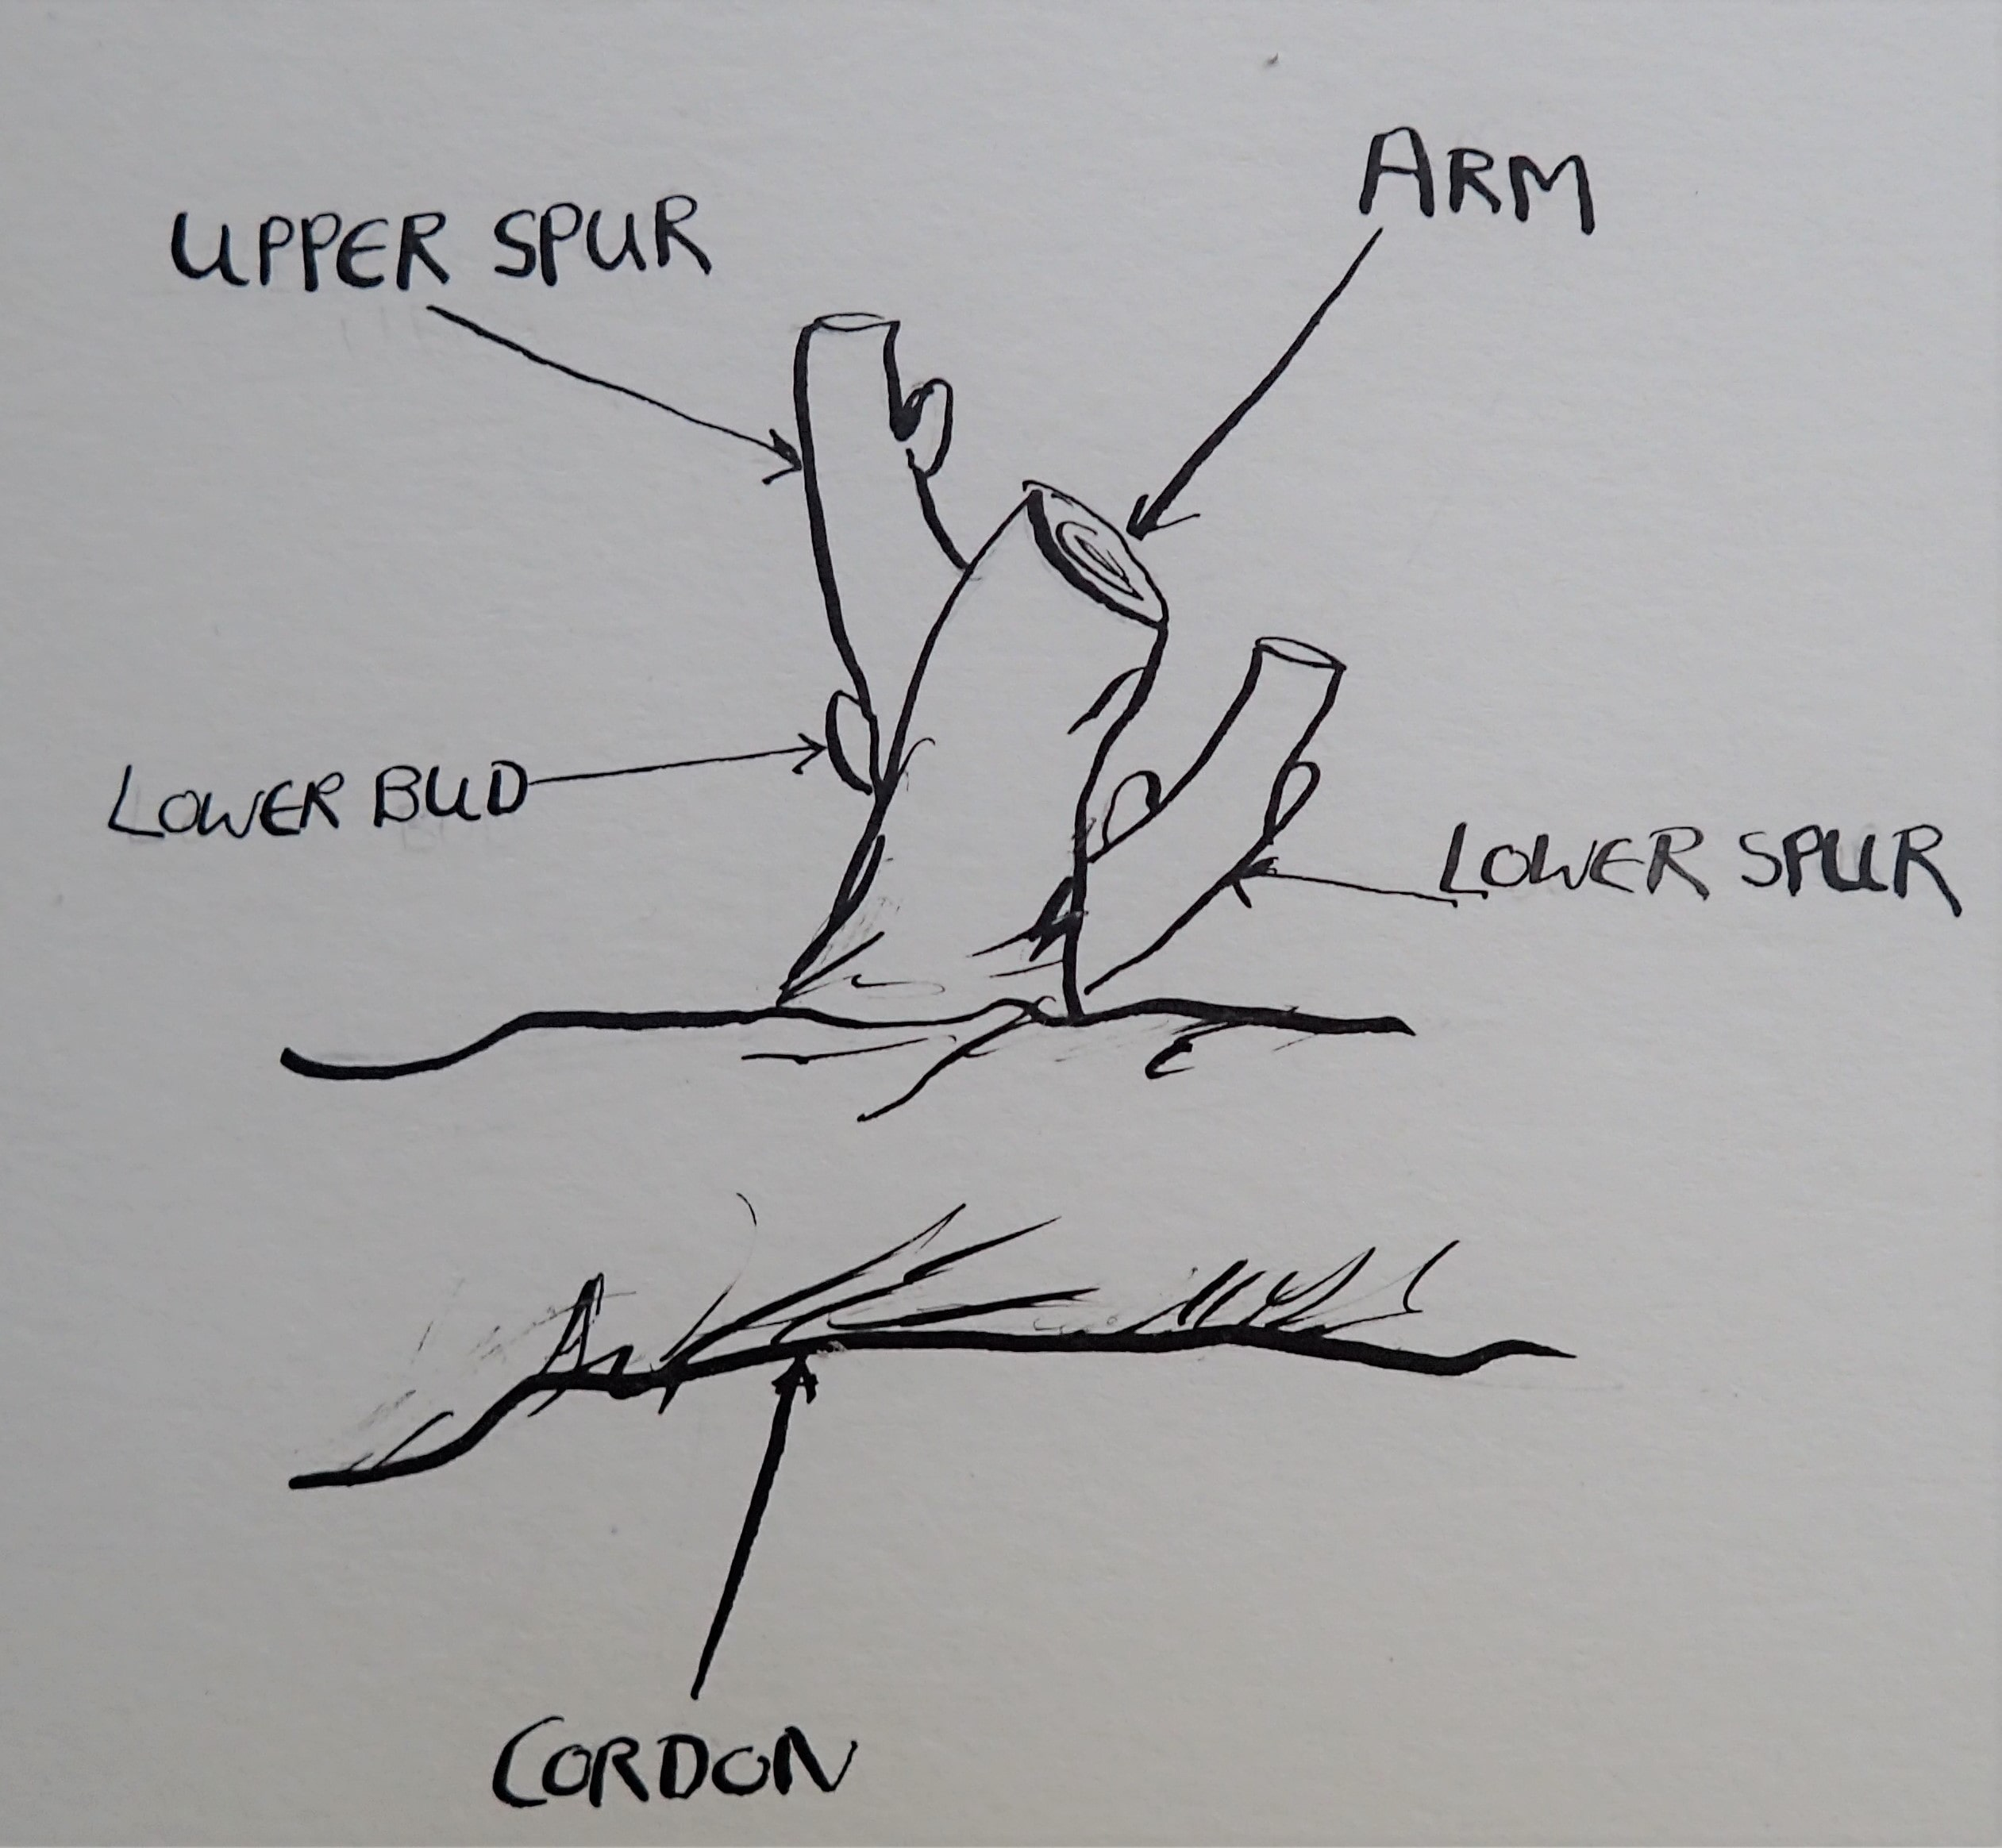
\includegraphics[width=\linewidth]{TwoSpurs.jpg}
  \caption{A diagram of an arm of a cordon that had two spurs on it. In this case we chose to focus on the lower bud of the higher of the two spurs for monitoring. }
  \label{fig:TwoSpurs}
\end{figure}



If plant was either cordon pruned (Figure \ref{fig:CordonPruned}) or cane pruned (Figure \ref{fig:CanePruned}, we flipped a coin to determine which side was flagged (heads = south or east, tails = north or west). If one side of the plant did not have enough buds, we chose the other side. If a plant had a cane and a cordon (Figure \ref{fig:CordonCane}, we flagged the cordon unless it did not have at least three spurs, then the cane was flagged. Occasionally, a cane would be trained back to the trunk in a loop or had come loose from the wire. (Figure \ref{fig:CaneCrossing}) In these cases, we flagged the other cane. If the cane started on one side but was trained to cross over and end on the other side, we used the direction of the end of the cane. 


\subsection{Cordon Buds}

We flagged the spur (or arm if it was present) on furthest from the trunk, a middle spur, and the first spur on the cordon with a base less than 5cm below the wire (Figure \ref{fig:CordonPruned}. Spurs more 5 or more centimeters below the wire were considered basal. If there was an even number of spurs, a coin flip determined which middle spur was chosen.

If there was more than one spur on an arm (Figure \ref{fig:TwoSpurs}) then we focused on the higher spur. We monitored the lowest bud on this spur. 

\subsection{Cane Buds}

We flagged the bud furthest from the trunk, the middle bud, and the first but that was farther than 15 centimeters from the trunk \ref{fig:CanePruned}. If there was an even number of middle buds, a coin flip determined which bud was chosen. 

If there were two buds in the same place in a position that was flagged, we chose to monitor the bud that was more upright. If both buds were equally upright facing, we monitored the one in a southerly or easterly direction. 

\section{Monitoring Buds}
We numbered the buds on each cordon or cane from 1 to 3, and numbered then in ascending order from either the south or the east (Figured \ref{fig:CordonPruned} and \ref{fig:CanePruned}. 

\section{Misc}
tape colors for QG are orange and blue, avoid flagging with these colors
Avoid orange and pink for Arterra - they seems to use of have most colors in their vineyards though
Ask vineyards at beginning of the season what color they prefer we use
Once at EL stage 7 or 9, flag bud itself?

\section{Contacting vineyards}

\end{document}